%\section{Introduction}
%\section{Why cointegration?}
\section{Why?}
% "Cointegration shared" ≈ long-term equilibrium
% "Cointegration correlated" ≈ Correlation in short-term behavior ≈ short-term dynamics

%How We Test for Unit RootsGoal: Before we can model our data, we must check if it's $I(0)$ or $I(1)$.The Test: We use a Unit-Root Test, such as the Augmented Dickey-Fuller (ADF) Test (Section 5.1.6).How it Works: The ADF test runs a regression like:$\Delta z_t = \beta z_{t-1} + \sum \phi_i^* \Delta z_{t-i} + a_t$Hypotheses:Null ($H_0$): $\beta = 0$ $\rightarrow$ The series has a unit root (it is $I(1)$).Alternative ($H_a$): $\beta < 0$ $\rightarrow$ The series is stationary (it is $I(0)$).Action: "For our project, we will first run the ADF test on all our variables. We expect to fail to reject the null, proving they are $I(1)$."

\begin{frame}{Problem}
	\textbf{How do we test for unit roots?}
	Goal?
\end{frame}

\begin{frame}[allowframebreaks]
	\frametitle{Unit roots testing}
	
	\textbf{Aim}: Check if the data is $I(0)$ or $I(1)$.
	
	\textbf{Test}: Augmented Dickey-Fuller (ADF) test
	
	\textbf{Method}: Run the following regression:
	$$\Delta z_t = \beta z_{t-1} + \sum \phi_i^* \Delta z_{t-i} + a_t$$
	
	\framebreak
	
	\textbf{Hypothesis testing}
	\begin{itemize}
		\item $H_0: \beta = 0 \rightarrow \exists$ a unit root ($I(1)$)
		\item $H_1: \beta < 0 \rightarrow$ stationary ($I(0)$)
	\end{itemize}
\end{frame}


\subsection{Problem}
\begin{frame}{Problem}
	%\textbf{Problem}
	\begin{center}
		Most real-world data are non-stationary.
	\end{center}
\end{frame}

\subsection{Trap}
\begin{frame}[allowframebreaks]
	\frametitle{The trap}
	
	\begin{figure}[H]
		\centering
		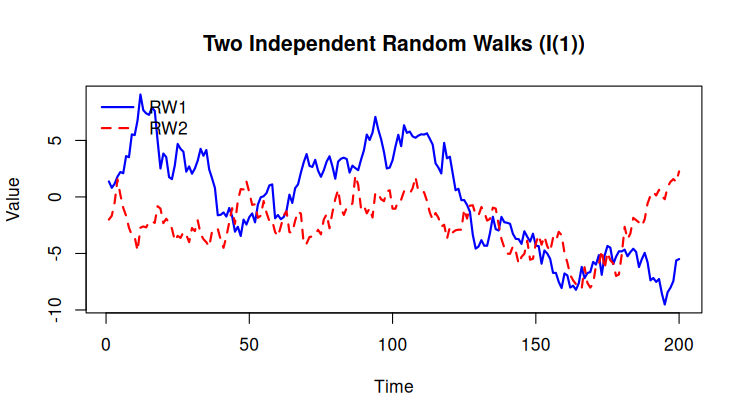
\includegraphics[width=\linewidth]{notes/twoRwalks.png}
		\caption{Two random walks}
	\end{figure}
	\framebreak
	
	%A \textbf{spurious regression} happens when you regress one non-stationary time series on another non-stationary time series that is not actually related.
	
	\begin{itemize}
		\item A \textbf{regression} may show a high R² and significant t-statistics, even though there is no real relationship between the variables.
		\item The regression is `\textbf{spurious}' or `\textbf{fake}'. It captures the common trends, not a true economic relationship. This is a major pitfall.
	\end{itemize}
	\framebreak
	
	\textbf{Example}:
	\small
	
	Suppose
	\begin{itemize}
		\item $X_t$ = global temperature over time
		\item $Y_t$ = stock prices over time
	\end{itemize}
	Both may increase over decades, so a regression explaining the phenomena would be:
	$$Y_t = \alpha + \beta X_t + \epsilon_t$$
	might show a very high $R^2$ and a significant $\beta$ due to its shared trend, not because of the variables affecting each other. But \texttt{temperatures} \& \texttt{stock prices} do not affect each other in real-world scenario. Hence this type of regression is called \textbf{spurious regression}.
\end{frame}

\begin{frame}[allowframebreaks]
	\frametitle{Correlation vs Cointegration}
	\begin{table}[h!]
		\centering
		\tiny
		\begin{tabular}{lll}
			\toprule
			
			\textbf{Feature} & \textbf{Correlation} & \textbf{Cointegration} \\ 
			
			\midrule
			
			\textbf{Time frame} & Short-term link & Long-term link \\ 
			
			\textbf{Type of data} & Works with any data & Needs non-stationary series \\ 
			
			\textbf{Focus} & Linear co-movement & Long-run equilibrium \\ 
			
			\textbf{Nature} & Simple dependence & Complex, involves stationarity \\ 
			
			\textbf{Example} & Two stocks move together & Oil and gas prices linked \\ 
			
			\bottomrule
		\end{tabular}
		\caption{Correlation vs. Cointegration comparison}
		\label{tab:corr__coint}
	\end{table}
\end{frame}

%\begin{frame}{Summary}
%	\begin{itemize}
%		\item \textbf{Correlation}: It is concerned with how two variables move together, but it is usually a \textit{short-term} or \textit{momentary measure}.
		
%		\item \textbf{Cointegration}: Deals with the long-term equilibrium between two non-stationary variables, implying that they share a common trend and are bound together in the long run.
%	\end{itemize}
%\end{frame}